\documentclass{standalone}
\usepackage{tikz}
\usepackage{verbatim}
\begin{document}
\pagestyle{empty}
  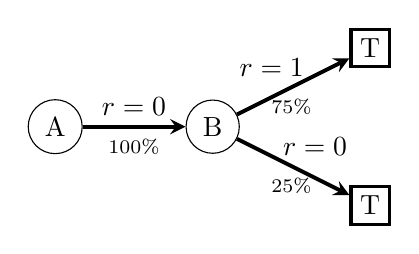
\begin{tikzpicture}
    \node[draw,circle] (a) at (0,0) {A};
    \node[draw,circle] (b) at (2,0) {B};
    \node[draw,rectangle, line width=0.4mm] (r1) at (4, 1) {T};
    \node[draw,rectangle, line width=0.4mm] (r0) at (4,-1) {T};
    \draw[-stealth, line width=0.5mm] (a) -- (b);
    \draw[-stealth, line width=0.5mm] (b) -- (r1);
    \draw[-stealth, line width=0.5mm] (b) -- (r0);
    \node at (1, 0.25) {$r=0$};
    \node at (1,-0.25) {$\scriptstyle 100\%$};
    \node at (2.75, 0.75) {$r=1$};
    \node at (3, 0.25) {$\scriptstyle 75\%$};
    \node at (3.3,-0.25) {$r=0$};
    \node at (3.0,-0.75) {$\scriptstyle 25\%$};
  \end{tikzpicture}
  \end{document}